\documentclass{standalone}
\usepackage{tikz}
\usetikzlibrary{patterns, positioning}

\begin{document}
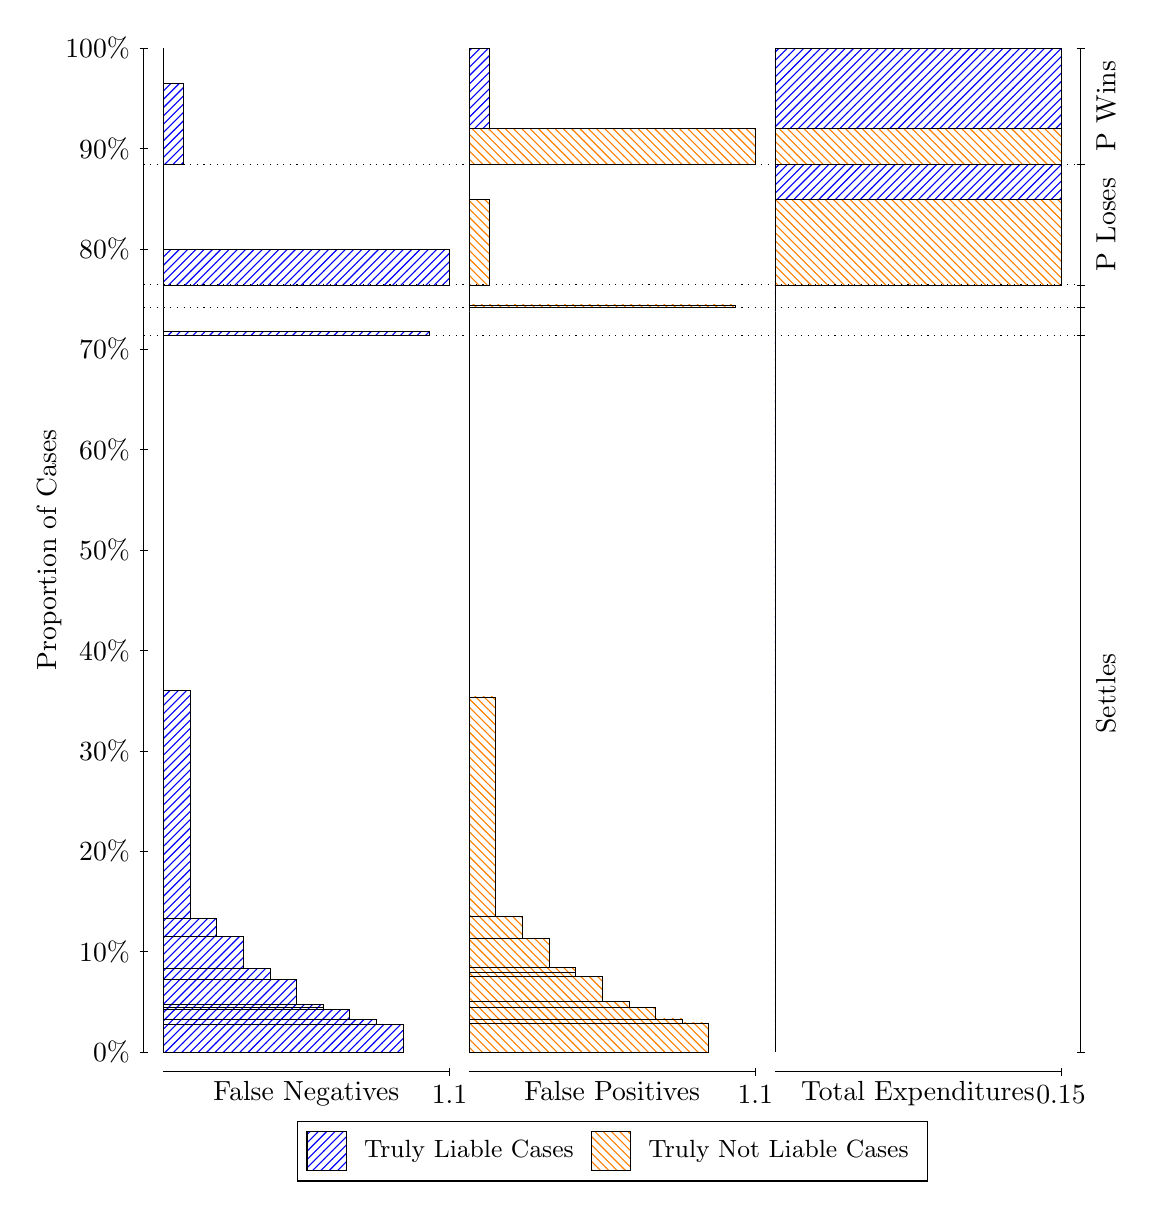
\begin{tikzpicture}
\draw[black, very thin] (1.5,1.75) -- (1.5,14.5);
\node[rotate=90, anchor=center] at (0.3, 8.125) {Proportion of Cases};
\draw[black, very thin] (1.45,1.75) -- (1.55,1.75);
\node[anchor=east] at (1.45, 1.75) {0\%};
\draw[black, very thin] (1.45,3.025) -- (1.55,3.025);
\node[anchor=east] at (1.45, 3.025) {10\%};
\draw[black, very thin] (1.45,4.3) -- (1.55,4.3);
\node[anchor=east] at (1.45, 4.3) {20\%};
\draw[black, very thin] (1.45,5.575) -- (1.55,5.575);
\node[anchor=east] at (1.45, 5.575) {30\%};
\draw[black, very thin] (1.45,6.85) -- (1.55,6.85);
\node[anchor=east] at (1.45, 6.85) {40\%};
\draw[black, very thin] (1.45,8.125) -- (1.55,8.125);
\node[anchor=east] at (1.45, 8.125) {50\%};
\draw[black, very thin] (1.45,9.4) -- (1.55,9.4);
\node[anchor=east] at (1.45, 9.4) {60\%};
\draw[black, very thin] (1.45,10.675) -- (1.55,10.675);
\node[anchor=east] at (1.45, 10.675) {70\%};
\draw[black, very thin] (1.45,11.95) -- (1.55,11.95);
\node[anchor=east] at (1.45, 11.95) {80\%};
\draw[black, very thin] (1.45,13.225) -- (1.55,13.225);
\node[anchor=east] at (1.45, 13.225) {90\%};
\draw[black, very thin] (1.45,14.5) -- (1.55,14.5);
\node[anchor=east] at (1.45, 14.5) {100\%};

\draw[black, very thin] (13.4,1.75) -- (13.4,14.5);
\draw[black, very thin] (13.35,1.75) -- (13.45,1.75);
\node[anchor=west] at (13.35, 1.75) {};
\draw[black, very thin] (13.35,10.853) -- (13.45,10.853);
\node[anchor=west] at (13.35, 10.853) {};
\draw[black, very thin] (13.35,11.204) -- (13.45,11.204);
\node[anchor=west] at (13.35, 11.204) {};
\draw[black, very thin] (13.35,11.493) -- (13.45,11.493);
\node[anchor=west] at (13.35, 11.493) {};
\draw[black, very thin] (13.35,13.025) -- (13.45,13.025);
\node[anchor=west] at (13.35, 13.025) {};
\draw[black, very thin] (13.35,14.5) -- (13.45,14.5);
\node[anchor=west] at (13.35, 14.5) {};

\draw[black, very thin, pattern color=blue, pattern=north east lines] (1.75,1.75) rectangle (4.7919,2.0957);
\draw[black, very thin, pattern color=blue, pattern=north east lines] (1.75,2.0957) rectangle (4.4539,2.1598);
\draw[black, very thin, pattern color=blue, pattern=north east lines] (1.75,2.1598) rectangle (4.1159,2.2926);
\draw[black, very thin, pattern color=blue, pattern=north east lines] (1.75,2.2926) rectangle (3.7779,2.3195);
\draw[black, very thin, pattern color=blue, pattern=north east lines] (1.75,2.3195) rectangle (3.7779,2.359);
\draw[black, very thin, pattern color=blue, pattern=north east lines] (1.75,2.359) rectangle (3.4399,2.6692);
\draw[black, very thin, pattern color=blue, pattern=north east lines] (1.75,2.6692) rectangle (3.1019,2.8152);
\draw[black, very thin, pattern color=blue, pattern=north east lines] (1.75,2.8152) rectangle (2.764,3.22);
\draw[black, very thin, pattern color=blue, pattern=north east lines] (1.75,3.22) rectangle (2.426,3.4426);
\draw[black, very thin, pattern color=blue, pattern=north east lines] (1.75,3.4426) rectangle (2.088,6.3438);
\draw[black, very thin, pattern color=orange, pattern=north west lines] (1.75,6.3438) rectangle (1.75,10.853);
\draw[black, very thin, pattern color=blue, pattern=north east lines] (1.75,10.853) rectangle (5.1298,10.904);
\draw[black, very thin, pattern color=orange, pattern=north west lines] (1.75,10.904) rectangle (1.75,11.204);
\draw[black, very thin, pattern color=orange, pattern=north west lines] (1.75,11.204) rectangle (1.75,11.239);
\draw[black, very thin, pattern color=blue, pattern=north east lines] (1.75,11.239) rectangle (1.75,11.493);
\draw[black, very thin, pattern color=blue, pattern=north east lines] (1.75,11.493) rectangle (5.3833,11.943);
\draw[black, very thin, pattern color=orange, pattern=north west lines] (1.75,11.943) rectangle (1.75,13.025);
\draw[black, very thin, pattern color=blue, pattern=north east lines] (1.75,13.025) rectangle (2.0035,14.05);
\draw[black, very thin, pattern color=orange, pattern=north west lines] (1.75,14.05) rectangle (1.75,14.5);
\draw[black, very thin, pattern color=orange, pattern=north west lines] (5.6333,1.75) rectangle (8.6752,2.1195);
\draw[black, very thin, pattern color=orange, pattern=north west lines] (5.6333,2.1195) rectangle (8.3372,2.1699);
\draw[black, very thin, pattern color=orange, pattern=north west lines] (5.6333,2.1699) rectangle (7.9992,2.3195);
\draw[black, very thin, pattern color=orange, pattern=north west lines] (5.6333,2.3195) rectangle (7.6612,2.3942);
\draw[black, very thin, pattern color=orange, pattern=north west lines] (5.6333,2.3942) rectangle (7.3233,2.7102);
\draw[black, very thin, pattern color=orange, pattern=north west lines] (5.6333,2.7102) rectangle (6.9853,2.7582);
\draw[black, very thin, pattern color=orange, pattern=north west lines] (5.6333,2.7582) rectangle (6.9853,2.8275);
\draw[black, very thin, pattern color=orange, pattern=north west lines] (5.6333,2.8275) rectangle (6.6473,3.1877);
\draw[black, very thin, pattern color=orange, pattern=north west lines] (5.6333,3.1877) rectangle (6.3093,3.4727);
\draw[black, very thin, pattern color=orange, pattern=north west lines] (5.6333,3.4727) rectangle (5.9713,6.2588);
\draw[black, very thin, pattern color=blue, pattern=north east lines] (5.6333,6.2588) rectangle (5.6333,10.853);
\draw[black, very thin, pattern color=orange, pattern=north west lines] (5.6333,10.853) rectangle (5.6333,11.152);
\draw[black, very thin, pattern color=blue, pattern=north east lines] (5.6333,11.152) rectangle (5.6333,11.204);
\draw[black, very thin, pattern color=orange, pattern=north west lines] (5.6333,11.204) rectangle (9.0132,11.239);
\draw[black, very thin, pattern color=blue, pattern=north east lines] (5.6333,11.239) rectangle (5.6333,11.493);
\draw[black, very thin, pattern color=orange, pattern=north west lines] (5.6333,11.493) rectangle (5.8868,12.574);
\draw[black, very thin, pattern color=blue, pattern=north east lines] (5.6333,12.574) rectangle (5.6333,13.025);
\draw[black, very thin, pattern color=orange, pattern=north west lines] (5.6333,13.025) rectangle (9.2667,13.475);
\draw[black, very thin, pattern color=blue, pattern=north east lines] (5.6333,13.475) rectangle (5.8868,14.5);
\draw[black, very thin, pattern color=orange, pattern=north west lines] (9.5167,1.75) rectangle (9.5167,6.2588);
\draw[black, very thin, pattern color=blue, pattern=north east lines] (9.5167,6.2588) rectangle (9.5167,10.853);
\draw[black, very thin, pattern color=orange, pattern=north west lines] (9.5167,10.853) rectangle (9.5167,11.152);
\draw[black, very thin, pattern color=blue, pattern=north east lines] (9.5167,11.152) rectangle (9.5167,11.204);
\draw[black, very thin, pattern color=orange, pattern=north west lines] (9.5167,11.204) rectangle (9.5167,11.239);
\draw[black, very thin, pattern color=blue, pattern=north east lines] (9.5167,11.239) rectangle (9.5167,11.493);
\draw[black, very thin, pattern color=orange, pattern=north west lines] (9.5167,11.493) rectangle (13.15,12.574);
\draw[black, very thin, pattern color=blue, pattern=north east lines] (9.5167,12.574) rectangle (13.15,13.025);
\draw[black, very thin, pattern color=orange, pattern=north west lines] (9.5167,13.025) rectangle (13.15,13.475);
\draw[black, very thin, pattern color=blue, pattern=north east lines] (9.5167,13.475) rectangle (13.15,14.5);
\draw[black, dotted] (1.5,10.853) -- (13.4,10.853);
\draw[black, dotted] (1.5,11.204) -- (13.4,11.204);
\draw[black, dotted] (1.5,11.493) -- (13.4,11.493);
\draw[black, dotted] (1.5,13.025) -- (13.4,13.025);
\draw[black, very thin] (1.75,1.5) -- (5.3833,1.5);
\node[anchor=north] at (3.5667, 1.5) {False Negatives};
\draw[black, very thin] (5.3833,1.45) -- (5.3833,1.55);
\node[anchor=north] at (5.3833, 1.45) {1.1};

\draw[black, very thin] (5.6333,1.5) -- (9.2667,1.5);
\node[anchor=north] at (7.45, 1.5) {False Positives};
\draw[black, very thin] (9.2667,1.45) -- (9.2667,1.55);
\node[anchor=north] at (9.2667, 1.45) {1.1};

\draw[black, very thin] (9.5167,1.5) -- (13.15,1.5);
\node[anchor=north] at (11.333, 1.5) {Total Expenditures};
\draw[black, very thin] (13.15,1.45) -- (13.15,1.55);
\node[anchor=north] at (13.15, 1.45) {0.15};

\node[black, centered, rotate=90] at (13.72, 6.3013) {Settles};


\node[black, centered, rotate=90] at (13.72, 12.259) {P Loses};
\node[black, centered, rotate=90] at (13.72, 13.762) {P Wins};

\draw (7.449999999999999,1.5) node[draw=none] (baseCoordinate) {};
\begin{scope}[align=center]
        \matrix[scale=0.5, draw=black, below=0.5cm of baseCoordinate, nodes={draw}, column sep=0.1cm]{
            \node[rectangle, draw, minimum width=0.5cm, minimum height=0.5cm, pattern=north east lines, pattern color=blue] {}; &
            \node[draw=none, font=\small] (B) {Truly Liable Cases}; &
            \node[rectangle, draw, minimum width=0.5cm, minimum height=0.5cm, pattern=north west lines, pattern color=orange] {}; &
            \node[draw=none, font=\small] (B) {Truly Not Liable Cases}; \\
            };
\end{scope}

\end{tikzpicture}
\end{document}